\documentclass[10pt,twocolumn]{article}
\usepackage{amsthm, amssymb, geometry, mathrsfs}
\usepackage[T1]{fontenc}
\usepackage{graphicx}
\usepackage[utf8]{inputenc}
\usepackage{multicol}% http://ctan.org/pkg/multicols

\title {COMP 598: Something Something Reddit}
\author {Xavier Denis, Ian Forbes, Liu Liu}

\begin {document}

\twocolumn[
\maketitle
\section{Abstract}
We collected a new machine learning dataset from the online social network Reddit. The dataset consisted of the top 100 posts from 2014, along with their comments from 10 subreddits. We implemented a naive Bayes classifier to classify the subreddit which the comment belongs. The binary classification performance of the naive Bayes was 89\% from 10-fold cross validation with around 700 comments. The multi-class classification performance with 6 classes using 150-900 comments per class was 75\%. This work can be potentially useful in the future to implement an algorithm to recommend subreddit for users based on their comment histories.
\\
\\
]
\section{What is Reddit?}

Reddit is a popular online link aggregation website. It allows user to post links to other webpages, images, videos, and more and to vote on the popularity of these submissions. Popular submissions are `Upvoted' while unpopular ones are `Downvoted'. Users are also allowed to comment on and discuss submissions. Comments, like submissions, are also subject to be voted on. Some of the key vocabulary of reddit is listed below.

\begin {enumerate}
\item \textbf{post:} Also know as a submission is a link to another webpage. This webpage may be a news article, a blog post, an image, a video, etc. All posts contain a comment section where user are allowed to discuss the submission.
\item \textbf{self post:} Is a special type of post where a user writes their own text submission. This is often used to started discussions or ask questions in a given subreddit. 
\item \textbf{subreddit:} A subsection of reddit dedicated to a certain topic. 
\item \textbf{upvote \& downvote:} The action of voting on the popularity of a comment in either a positive or negative manner.
\item \textbf{top level comment:} The root of a comment tree.
\end {enumerate}

\section{Motivation}
With the rise of social networks, many researchers have poured over the data produced to find explore the connections between friends, text, and social interactions. While much research has been done on networks such as Twitter and Facebook, Reddit has remained largely ignored. The different structure of Reddit allows for an opportunity to look at different questions and a different style of conversation. Because Reddit users can label comments and posts as good or bad by voting, we can attempt to predict the interests of reddit users. 

One advantage of using Reddit as a data source is that one, all content is publicly available, and two, it has an easy to use REST API. 

\begin{figure*}
    \centering
  	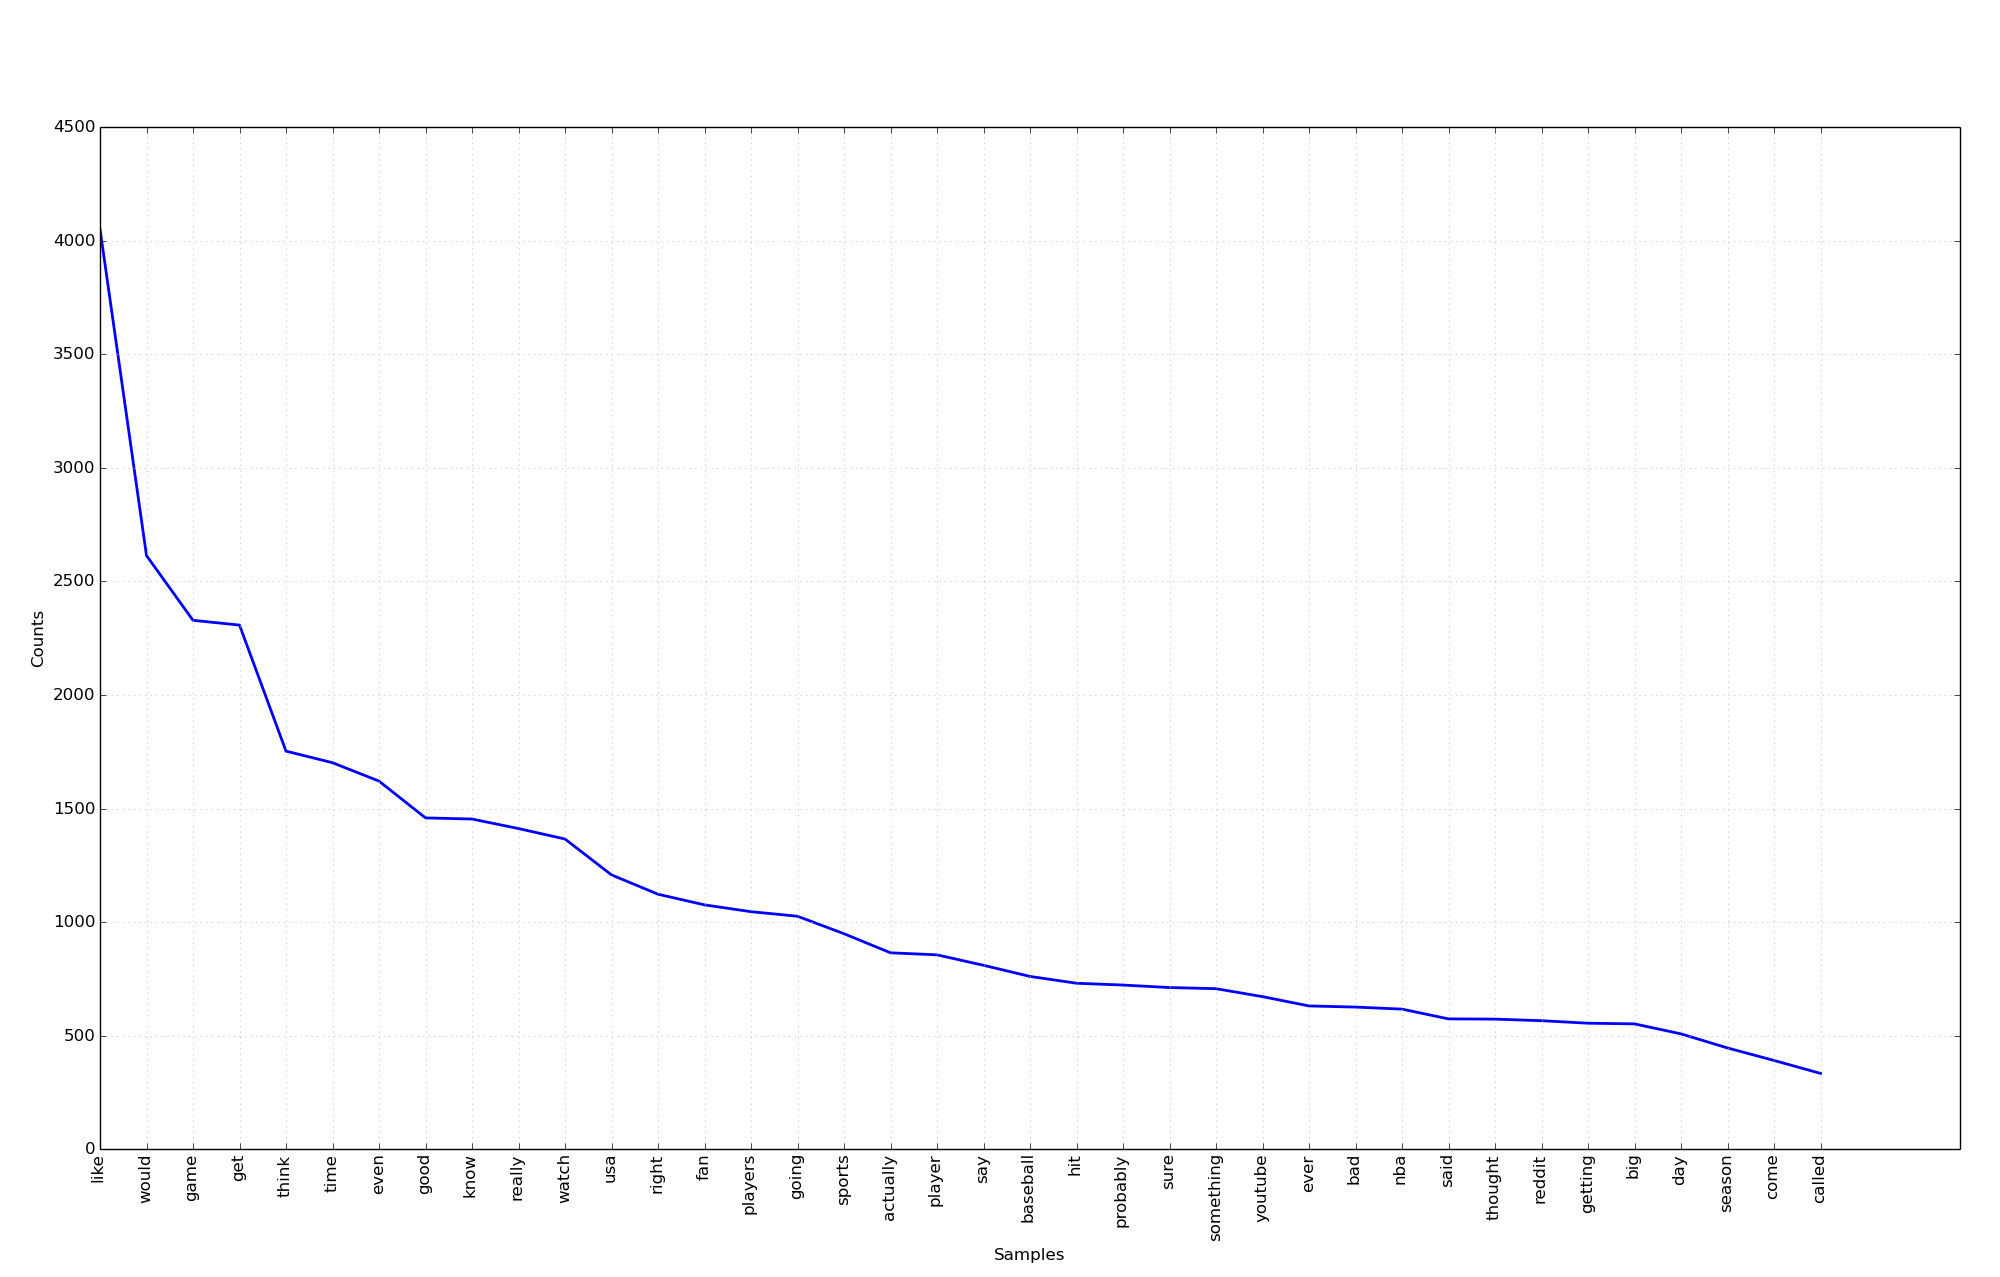
\includegraphics[width=0.92\textwidth]{./sports_freq.png}
  	\caption{Word frequency of the Sports subreddit.}
  	\label{fig:RSUencountered}
\end{figure*}

\section{Related Work}
Due to the lack of studies related to Reddit there are few related datasets or papers. A search through Google Scholar produces few results and the top links are only listed because of share buttons on the paper's hosting site. Most of the related research we found was University projects like our own. We could not find any published papers or data.

That being said we did find an interesting analysis that aimed to predict the popularity of a self post based on its Flesch-Kincaid readability. This project found a correlation between how easy a self post was to read and how popular it would be. In particular posts with moderate readability where more popular than others with easy or hard readability.

\section{Dataset Description}

Reddit's developer API allowed us to download all of the post and comments data into a structured JSON file. Each post is saved in a JSON file under its primary identifier. Each date file consists of 2 main parts, the meta data and the comments. The meta data contains information about the post, such as how many comments there are, the score of the post, a link to the content and the type of content (image, video, article, etc.). The comments section consists of a list the top level comments for that post. Each of the top level comments contains a list of of child comments (replies) which in turn may have their own children. This forms a recursive tree structure with the top level post as the root. 

In order to train our naive Bayes classifier we had to flatten the comments and evaluate the word frequency in each post, this can be done using a simple tree traversal algorithm that can be found in the appendix. 

\section{Methods}
Naive Bayes Classifier
The motivation for using Naive Bayes text classifier is that the text data has many features. i.e. since there are many possible words, and not too many text posts and comments in the data from Reddit. Therefore, the combination of words will not likely to appear in the text data to generate models of P(x|y) and apply generative learning (e.g. LDA) to text data classification.
Naive Bayes assume the $x$ are conditionally independent given $y$ and simplifies the problem.
[Insert tree diagram]
Laplace smoothing was applied since some words are not observed in the training data. The maximum likelihood estimator was,
\[
P(x_j|y=1) = \frac {\#[x_j=1 \land y=1]+1}{\#[y=1]+2}
\]
Therefore, if there are no words from that class, the prior probability will be $0.5$

\section{Results}
		
\section{Discussion}
The final dataset and features are accurate when classifying but could still be improved. There were several issues during tokenization where standard approaches would fail due to reddit's internal culture. The frequent use of non-textual unicode characters to encode emojis and other information wouldn't be captured by pure word tokenization. Additionally, the presence of Markdown for text formatting adds another level of complexity to the word extraction. We settled on stripping markdown formatting through regexes before splitting on spaces and stemming words. However, there a few issues with things such as `l33tspeak' where numbers are subsistuted for letters, causing use to not recognize identical words. 

Overall our results were quite positive. On possible use of our classifier would be to recommend new subreddits to users based on their comment history. Each user's comments are publicly available on their profile so it would be very easy to classify each of the comments into a given subreddit. If a user's comments where consistently classified into a small subset of subreddits it is possble that they may be interested in that subreddit. On a larger scale, sometimes posts are added to the wrong subreddit, this classifier could detect that comments really belong in a different subreddit and automatically move the entire post to that subreddit where it could recieve the apropriate community interaction.

We hereby state that all the work presented in the report is that of the authors.

\section{References}

\section{Appendix}

\end{document}